%% 该模板修改自《计算机学报》latex 模板
%% 主要是将双栏改成单栏,去掉了部分计算机学报标识;
%% 源文件自:https://www.overleaf.com/latex/templates/latextemplet-cjc-xelatex/ybmmymncrrmw
%% 
%%
%% This is file `CjC_template_tex.tex',
%% is modified by Zhi Wang (zhiwang@ieee.org) based on the template 
%% provided by Chinese Journal of Computers (http://cjc.ict.ac.cn/).
%%
%% This version is capable with Overleaf (XeLaTeX).
%%
%% Update date: 2023/03/10
%% -------------------------------------------------------------------
%% Copyright (C) 2016--2023 
%% -------------------------------------------------------------------
%% This file may be distributed and/or modified under the
%% conditions of the LaTeX Project Public License, either version 1.3c
%% of this license or (at your option) any later version.
%% The latest version of this license is in
%%    https://www.latex-project.org/lppl.txt
%% and version 1.3c or later is part of all distributions of LaTeX
%% version 2008 or later.
%% -------------------------------------------------------------------

\documentclass[10.5pt,compsoc,UTF8]{CjC}
\usepackage{CTEX}
\usepackage{graphicx}
\usepackage{footmisc}
\usepackage{subfigure}
\usepackage{url}
\usepackage{multirow}
\usepackage{multicol}
\usepackage[noadjust]{cite}
\usepackage{amsmath,amsthm}
\usepackage{amssymb,amsfonts}
\usepackage{booktabs}
\usepackage{color}
\usepackage{ccaption}
\usepackage{booktabs}
\usepackage{float}
\usepackage{fancyhdr}
\usepackage{caption}
\usepackage{xcolor,stfloats}
\usepackage{comment}
\setcounter{page}{1}
\graphicspath{{figures/}}
\usepackage{cuted}%flushend,
\usepackage{captionhack}
\usepackage{epstopdf}
\usepackage{gbt7714}
\usepackage{listings}
\usepackage{xeCJK}
\usepackage{float}
\usepackage{sourcecodepro}
\usepackage[T1]{fontenc}
\usepackage{hyperref}

\setmainfont{Times Roman}
% \setCJKmainfont{Noto Sans Mono CJK TC}
\setCJKmainfont{標楷體.ttc}
\setmonofont{Cascadia Code}

%===============================%

\headevenname{\mbox{\quad} \hfill  \mbox{\zihao{-5}{ \hfill 2024 Hardware Design  } \hspace {50mm} \mbox{2024 年 2 月}}}%
\headoddname{Group 21 \hfill Lab 1: Gate-Level Verilog}%

%footnote use of *
\renewcommand{\thefootnote}{\fnsymbol{footnote}}
\setcounter{footnote}{0}
\renewcommand\footnotelayout{\zihao{5-}}

\newtheoremstyle{mystyle}{0pt}{0pt}{\normalfont}{1em}{\bf}{}{1em}{}
\theoremstyle{mystyle}
\renewcommand\figurename{figure~}
\renewcommand{\thesubfigure}{(\alph{subfigure})}
\newcommand{\upcite}[1]{\textsuperscript{\cite{#1}}}
\renewcommand{\labelenumi}{(\arabic{enumi})}
\newcommand{\tabincell}[2]{\begin{tabular}{@{}#1@{}}#2\end{tabular}}
\newcommand{\abc}{\color{white}\vrule width 2pt}
\renewcommand{\bibsection}{}
\makeatletter
\renewcommand{\@biblabel}[1]{[#1]\hfill}
\makeatother
\setlength\parindent{2em}
%\renewcommand{\hth}{\begin{CJK*}{UTF8}{gbsn}}
%\renewcommand{\htss}{\begin{CJK*}{UTF8}{gbsn}}
\renewcommand{\contentsname}{Table of Contents}

\begin{document}

\hyphenpenalty=50000
\makeatletter
\newcommand\mysmall{\@setfontsize\mysmall{7}{9.5}}
\newenvironment{tablehere}
  {\def\@captype{table}}

\let\temp\footnote
\renewcommand \footnote[1]{\temp{\zihao{-5}#1}}

\hypersetup{
  colorlinks=false,
  pdfborder={0 0 0},
}

\thispagestyle{plain}%
\thispagestyle{empty}%
\pagestyle{CjCheadings}

% \begin{table*}[!t]
\vspace {-13mm}


\onecolumn
\zihao{5-}\noindent Group 21 \hfill Lab 1: Gate-Level Verilog \hfill 2024 年 2 月\\
\noindent\rule[0.25\baselineskip]{\textwidth}{1pt}


\begin{center}
    \vspace {11mm}
    {\zihao{2} \heiti \fangsong Lab 1: Gate-Level Verilog }
    
    \vskip 5mm
    
    {\zihao{4}\fangsong Group 21: 陳克盈(112062205)、蔡明妡(112062224)}
\end{center}

\lstset{
    % backgroundcolor=\color{red!50!green!50!blue!50},%程式碼塊背景色為淺灰色
    rulesepcolor= \color{gray}, %程式碼塊邊框顏色
    breaklines=true,  %程式碼過長則換行
    numbers=left, %行號在左側顯示
    numberstyle= \small\ttfamily,%行號字型
    keywordstyle= \color{blue},%關鍵字顏色
    commentstyle=\color{gray}, %註釋顏色
    frame=shadowbox%用方框框住程式碼塊
    basicstyle=\ttfamily\footnotesize,
}
 
\definecolor{improvecolor}{rgb}{0,0.6,0} % 深綠色
\definecolor{declinecolor}{rgb}{0.6,0,0} % 深紅色


%%%%%%%%%%%%%%%%%%%%%%%%%%%%%%%%%%%%%%
\zihao{5}
\vskip 10mm
% \begin{multicols}{1}


%%%%%%%%%%%%%%%%%%%%%%%%%%%%%%%%%%%%%%%%%%
%%%%%%%%%%%%%%%%%%%%%%%%%%%%%%%%%%%%%%%%%%

\tableofcontents
\newpage

\section{Lab 1: Gate-Level Verilog}
這部分附上在 Lab 時實作的 module circuit,這些電路將會被用來實作之後的題目。

\begin{figure}[h]
    \centering
    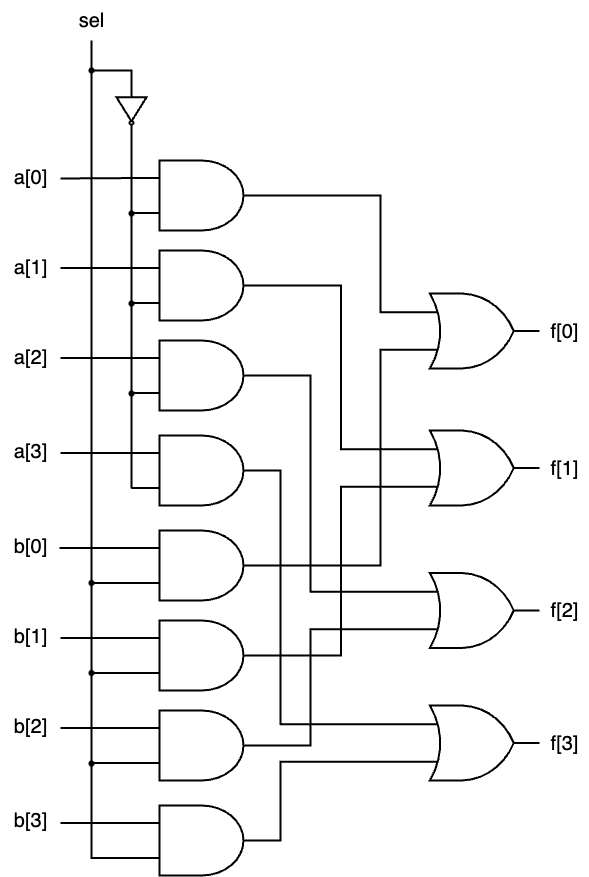
\includegraphics[width=0.5\textwidth]{2-to-1 MUX.png}
      \caption{2-to-1 MUX circuit}
    \label{fig:1-to-2-MUX}
\end{figure}

\newpage

\begin{figure}[h]
    \centering
    
\includegraphics[width=0.5\textwidth]{D_Latch.png}
      \caption{D-Latch circuit}
    \label{fig:D-Latch}
\end{figure}

\begin{figure}[h]
    \centering
    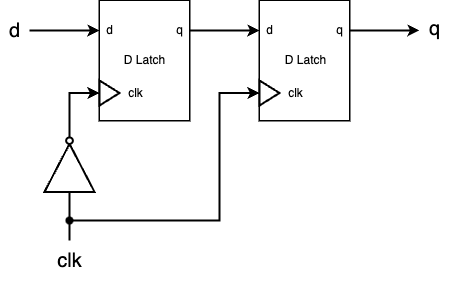
\includegraphics[width=0.6\textwidth]{D_Flip_Flop.png}
      \caption{D-Flip-Flop circuit}
    \label{fig:D-Flip-Flop}
\end{figure}

\section{Q1: 4-bit 1-to-4 de-multiplexer (DMUX)}
% \lipsum[1]

\subsection{Requirement}
Q1 要求使用三個\ 4-bit 1-to-2 的 DMUX 實作一個\ 4-bit 1-to-4 的 DMUX,基本運作原理就跟\ MUX 相反,透過\ select bit,將輸入輸出到對應的輸出線。

  

\subsection{Implement \& Circuit}
\subsubsection*{1-to-2 DMUX}

input: $in, sel$, output: $a, b$
\par

透過 \ $X \& 0 = 0, X \& 1 = X$ 的性質,將\ $a$ 與\ $in \& !sel$ 做 AND,代表當\ $sel = 0$ 時,$a$ 的值是\ $in$,反之則為\ $0$。而\ $b$ 則是與\ $in \& sel$ 做 AND,就能得到當\ $sel = 1$ 時,$b$ 的值是\ $in$,反之則為\ $0$ 的效果,如此一來便完成了這個 1-to-2 的 DMUX。

\begin{figure}[h]
    \centering
    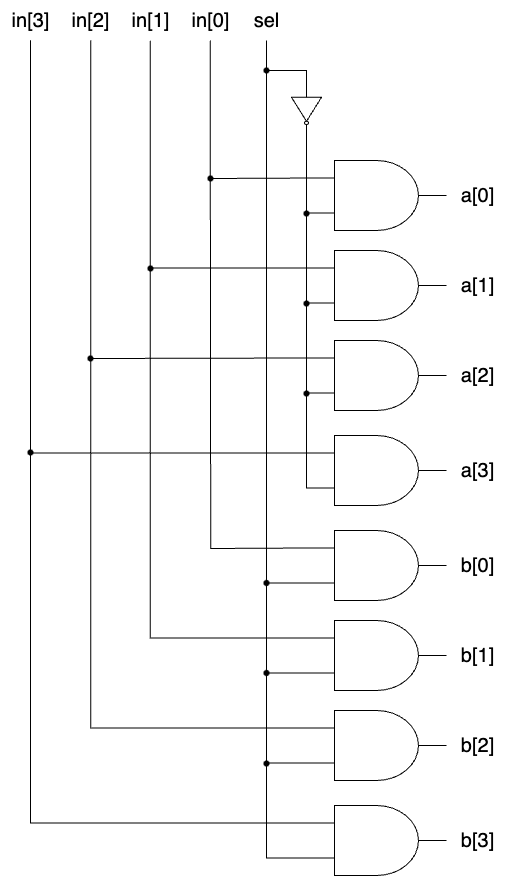
\includegraphics[width=0.4\textwidth]{1-to-2 DMUX.png}
      \caption{1-to-2 DMUX circuit}
    \label{fig:1-to-2-DMUX}
\end{figure}

\subsubsection*{1-to-4 DMUX}

input: $in, sel$, output: $a, b, c, d$
\par

利用二進位的性質,先將 $a, b, c, d$ 分成 $ab, cd$ 兩組。利用一個 1-to-2 DMUX,利用 sel[1] 作為 select bit 判斷出輸入應該要被重導向到 $ab$ 或是 $cd$。
\par
最後再個別將 $ab$, $cd$ 利用 sel[0] 作為 select bit 就能夠成功的重導向至 $a, b, c, d$ 了。

\begin{figure}[h]
    \centering
    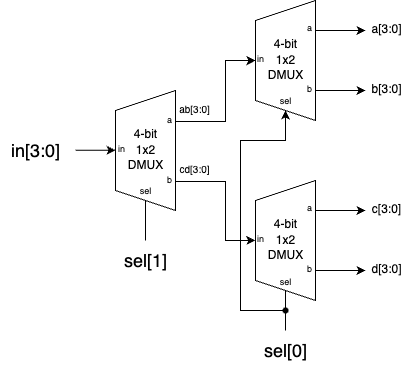
\includegraphics[width=0.5\textwidth]{1-to-4 DMUX.png}
      \caption{1-to-4 DMUX circuit}
    \label{fig:1-to-4-DMUX}
\end{figure}

\subsection{Testbench}
由於只有導向 $a / b / c / d$ 四種狀態,因此只需要將 $sel$ 做四次循環,每次做完就 $+1$ 就能夠遍歷所有狀態了。
\par
為了更清楚地看出輸入被導向哪一條線路,實際撰寫 Testbench 的時候是讓 $sel$ 做八次循環,並且每次做完都將 $in + 1$。
\par
從圖\ref{fig:DMUX_wave} 可以看出,隨著 $sel$ 的變動,$a, b, c, d$ 會輪流接收到 $in$ 的值。

\begin{figure}[h]
    \centering
    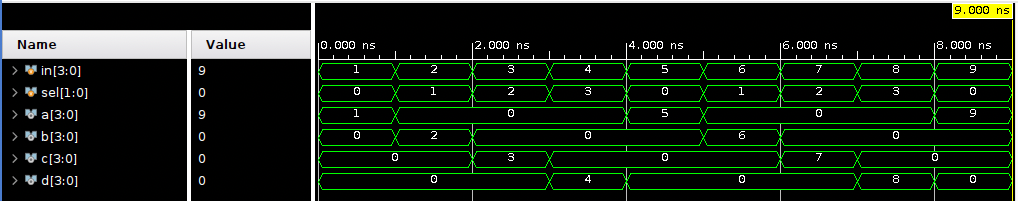
\includegraphics[width=\textwidth]{DMUX_wave.png}
      \caption{DMUX wave}
    \label{fig:DMUX_wave}
\end{figure}

\section{Q2: 4-bit simple crossbar switch with MUX/DMUX}

\subsection{Requirement}

根據所給的架構圖(圖 \ref{fig:2x2_spec})實現一個 4-bit 的 crossbar,當 $control = 1$ 時,需要將兩筆資料的輸出反轉,否則不變。

\begin{figure}
    \centering
    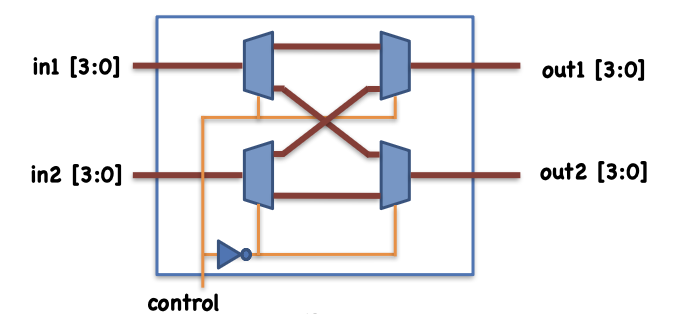
\includegraphics[width=\textwidth]{2x2_spec.png}
      \caption{2x2 crossbar arch}
    \label{fig:2x2_spec}
\end{figure}

\subsection{Implement \& Circuit}

根據架構圖,使用之前實作過的 1-to-2 DMUX 與 1-to-2 MUX 來實現。如此一來,在 $control = 0$ 時,$in1, in2$ 就會走原來的通道,\\
而當 $control = 1$ 時,則會走交叉的通道。
\par
關於此架構的推導方式補充在附錄(\ref{sec:crossbar})中。

\begin{figure}[h]
    \centering
    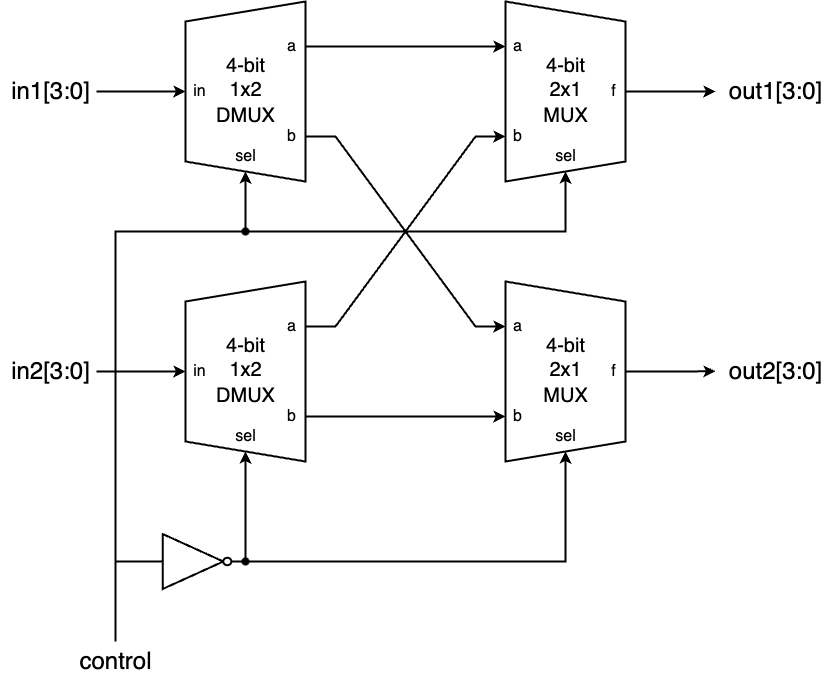
\includegraphics[width=0.5\textwidth]{2x2 crossbar.png}
      \caption{2x2 crossbar}
    \label{fig:2x2_crossbar}
\end{figure}


\subsection{Testbench}
由於只有兩種情況:$control = 0, control = 1$,因此只需要枚舉這兩個情況即可。
\par
不過為了更清楚地看出結果,我們採取了模擬 8 次,並在 $in1 = 0, in2 = 2$ 的初始狀態下,每次將 $in1, in2$ 分別 $+1$。 
\par
從圖\ref{fig:2x2_wave}中可以看出,隨著 $control$ 的變動,$out1, out2$ 的值會不斷地交換。

\begin{figure}[h]
    \centering
    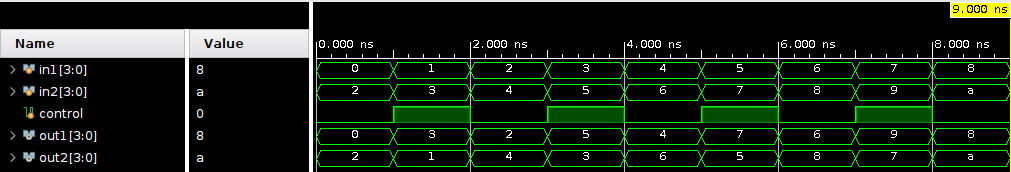
\includegraphics[width=\textwidth]{2x2_wave.png}
      \caption{2x2 crossbar wave}
    \label{fig:2x2_wave}
\end{figure}

\section{Q3: 4-bit 4x4crossbar with simple crossbar switch}

\subsection{Requirement}
根據題目給的架構圖(圖 \ref{fig:4x4_spec}),利用五個 2x2 crossbar 實作出 4x4 crossbar。

\begin{figure}[h]
    \centering
    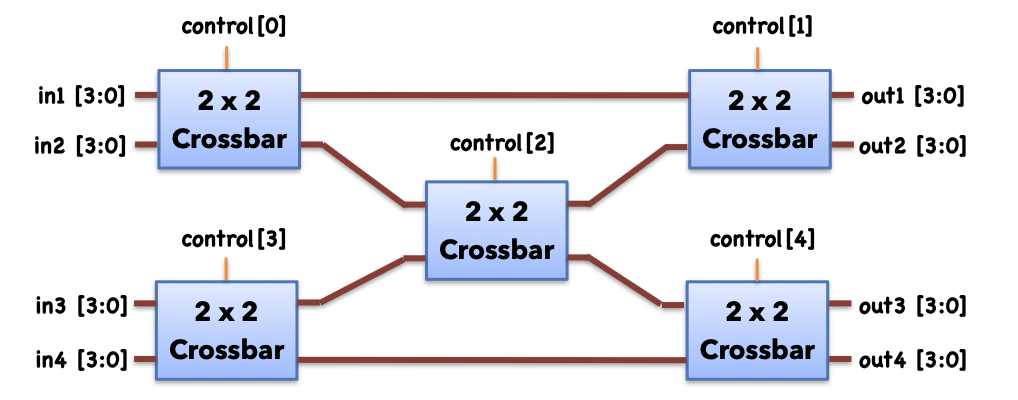
\includegraphics[width=\textwidth]{4x4_spec.png}
      \caption{4x4 crossbar arch}
    \label{fig:4x4_spec}
\end{figure}

\subsection{Implement \& Circuit}
建立相對應的電路,並將其以架構圖中的結構相互連接。

\begin{figure}[!h]
    \centering
    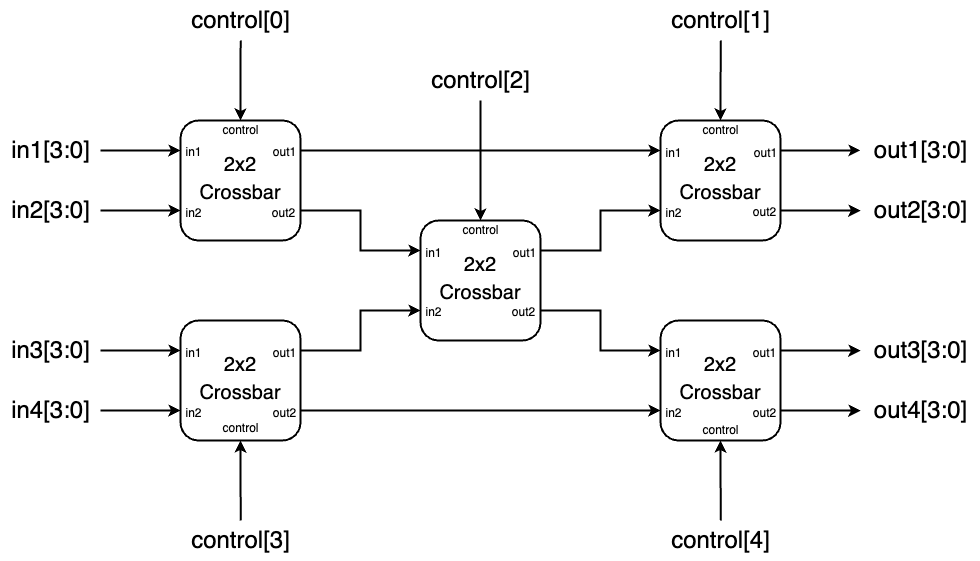
\includegraphics[width=\textwidth]{4x4 crossbar.png}
      \caption{4x4 crossbar circuit}
    \label{fig:4x4_crossbar}
\end{figure}

\newpage


\subsection{Benchmark}
枚舉 $control = 0 \sim 2^5 - 1$,以列出所有組合,並將 $in1, in2, in3, in4$ 分別設為 $1, 2, 3, 4$,以方便觀察不同 $control$ 之下,output 是如何對應 input 的。

\begin{figure}[h]
    \centering
    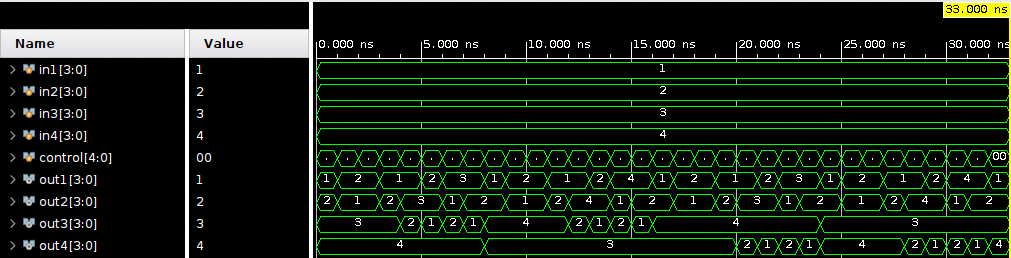
\includegraphics[width=\textwidth]{4x4_wave.png}
      \caption{4x4 crossbar wave}
    \label{fig:4x4_wave}
\end{figure}

\subsection{Combinations}

所有組合中,有 4 種沒有出現過:
\begin{enumerate}
    \item (3, 4, 1, 2)
    \item (3, 4, 2, 1)
    \item (4, 3, 1, 2)
    \item (4, 3, 2, 1)
\end{enumerate}

這是因為 $in1, in2$ 以及 $in3, in4$,都只有最多一個資料能夠透過 Crossbar 傳遞到一側,因此這四個組合不可能出現的。


\section{1-bit toggle flip flop (TFF)}
input: $clk, t, rst_n$, output: $q$

\subsection{Requirement}
依照所給的架構圖(圖 \ref{fig:TFF_spec}),利用 XOR, AND, D-Flip-Flop (DFF) 實作 T-Flip-Flop (TFF)

\begin{figure}[h]
    \centering
    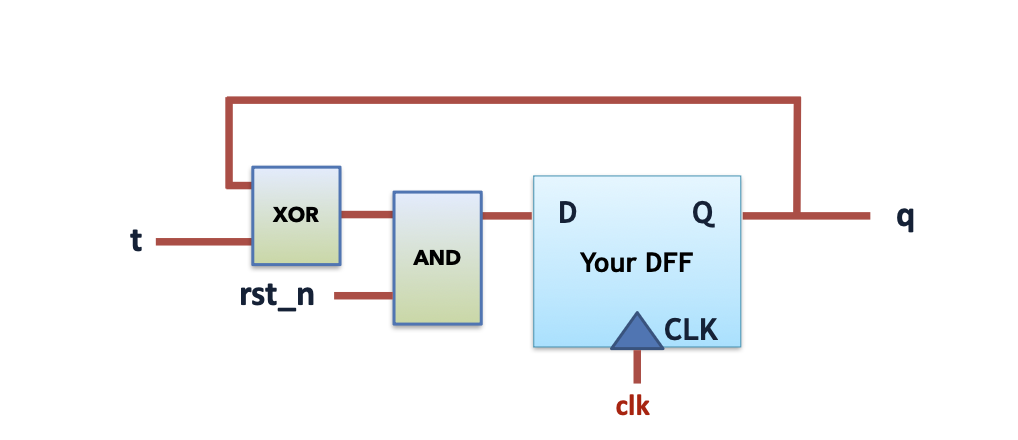
\includegraphics[width=\textwidth]{TFF_spec.png}
      \caption{TFF arch}
    \label{fig:TFF_spec}
\end{figure}

\subsection{Implement \& Circuit}

根據 $XOR(A, B) = (\bar{A}B + A\bar{B})$,先實作出 XOR,最後再依據架構圖以及之前寫過的 DFF 實現出 TFF。
\par
圖中的 $rst_n$ 代表著重設的訊號,當 $rst_n = 1$ 時,將不影響電路運作,但當 $rst_n = 0$ 時,無論上一個狀態為何,\\
都只會將 False 訊號傳遞至 D Flip-Flop,達到重設的效果。

\begin{figure}
    \centering
    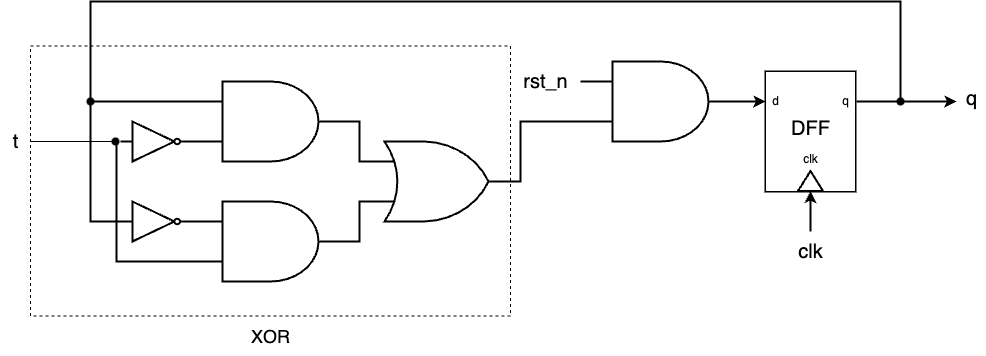
\includegraphics[width=\textwidth]{Toggle-D_Flip_Flop.png}
      \caption{TFF Circuit}
    \label{fig:TFF}
\end{figure}

\subsection{Testbench}

由於 TFF 的性質為:
\begin{itemize}
    \item 當 $rst_n = 0$ 時,重設輸出為 $0$,否則依照以下的規則運作
    \item 當 $T = 0$ 且 $clk$ 時脈往上時,輸出目前 $q$ 的反相
\end{itemize}

因此若是所有輸入都以相同的間隔切換,將會難以看出 TFF 的作用,因此採用了 $(clk, t, rst_n)$ 分別以 $(2ns, 3ns, 5ns)$ 的頻率同步,結果如下圖:
\par
由於此電路是以正緣作為觸發標準,所以可以觀察所有 $clk$ 從 $0 \rightarrow 1$ 的時間點,都符合了上述的 TFF 性質。

\begin{figure}[h]
    \centering
    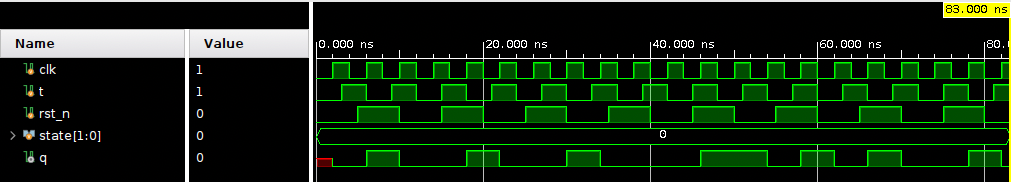
\includegraphics[width=\textwidth]{TFF_wave.png}
      \caption{TFF wave}
    \label{fig:TFF_wave}
\end{figure}

\section{FPGA Implementation}

\subsection{Requirement}
將 2x2 crossbar 實作在 FPGA 上,透過開關當作 input,LED 當作 output。跟原來的 2x2 不一樣的是,這次一個 output bit 會對應到兩個 LED 燈。

\subsection{Implement}
由於 vivado 不能直接將一個訊號 mapping 到兩個 LED 上,因此我們將原始的 2x2 crossbar 擴充,\\
$out1, out2$ 各複製一份出來,再將其透過 vivado 內的 IO Setting map 到所對應的 LED 上。

\section{Conclusion \& Discussion}

\subsection{2x2 crossbar 電路圖推導}\label{sec:crossbar}

總共會有四條線路需要實現,分別為:$in1 \rightarrow out1$, $in1 \rightarrow out2$, $in2 \rightarrow out1$, $in2 \rightarrow out2$,分別將這四條線路命名為 $A, B, C, D$
\par
首先利用兩個 1-to-2 DMUX 判斷 input 分別需要走到哪一條線路,DMUX1 分別接了 $in1, A, B$,而 DMUX2 接了 $in2, C, D$ 總共會有兩種情況:
\begin{enumerate}
    \item $control = 0$: $A, D$,此時 DMUX1 應該要輸出到第一個輸出,也就是 $A$,DMUX2 則是要輸出到第二個輸出,也就是 $D$
    \item $control = 1$: $B, C$,同理反之
\end{enumerate}
根據以上觀察,我們便可以得出 DMUX1 的 control bit 為 $control$,DMUX2 則為 $!control$
\par

接著是判斷 $out1, out2$ 分別是由哪一條線路提供,這邊可以使用 1-to-2 MUX 來實現。\\
MUX1 接了 $A, C$,MUX2 接了 $B, D$ 一樣有兩種情況:
\begin{enumerate}
    \item $control = 0$: $out1 = A, out2 = D$,此時 MUX1 需要輸出 $A$,MUX2 需要輸出 $D$
    \item $control = 1$: $out1 = B, out2 = C$,同理反之
\end{enumerate}
透過觀察,得出結論 MUX1 的 control bit 為 $control$,MUX2 的 control bit 則為 $!control$

\par

最後,將以上兩個結論,利用之前寫過的 DMUX 與 MUX,即可完成最終的目標

\subsection{我們學到了什麼、分工}

\subsubsection*{我們學到了什麼}

\begin{itemize}
    \item 如何安裝 Vivado:由於我們兩個都是使用 M2 MacBook Air,並不原生支援 Vivado,因此我們透過 Docker 模擬了 x86 環境下的 Linux\\
    再到這個環境下安裝 Vivado,並且有成功跑起來。
    \item 如何操作 Vivado:Vivado 在這門課主要有兩個用途,一個是用來跑 Testbench,模擬各種情況下,電路的輸出會是怎樣。\\
    另一個則是用來將電路實際燒錄到 FPGA 上,並且透過開關、LED 來觀察電路的運作。而後者又分成了幾個步驟:
    \begin{itemize}
        \item Run Synthesis: 將 Verilog code 編譯成一個 netlist。這個步驟結束後,我們就可以透過 IO Port 的設定工具,\\
        將 verilog 中的輸入輸出對應到 FPGA 上的 Port。除此之外,Vivado 也提供了查看電路圖的功能,可以讓我們初步的檢查電路是否如我們預期
        \item Run Implementation:這個步驟會根據我們所使用的硬體,將 netlist 近一步的優化、佈局、佈線等。
        \item Generate Bitstream:這個步驟會將最後的結果編譯成一個 bitstream,這個 bitstream 就是我們要燒錄到 FPGA 上的檔案。\\
        \item 大型應用的使用方式:在進行以上步驟的時候,都有能夠選擇要開幾個 process 的選項,這代表 Vivado 本身有支援平行計算。\\
        除此之外,Vivado 也支援了 remote host 的功能,我想或許在開發大型應用的時候,就是利用這個功能在伺服器上運算,\\
        最後再將生成的 bitstream 下載到本地端的 FPGA 上。
    \end{itemize}
    執行完這三個步驟後,就可以將 bitstream 燒錄到 FPGA 上,並且透過開關、LED 來觀察電路的運作。
    \item 對於 crossbar 的理解:在接觸這門課之前,我們對電子元件是如何切換資料路徑感到困惑,畢竟處理器只是由許多固定的電路組成,\\
    並不存在實體的開關來調節資料流。透過這次的實作,雖然應用面可能更複雜,但至少我理解了他的基本概念。
    \item Testbench 的理解與實作:這次實作了多個 Testbench,除了需要枚舉所有狀態之外,也需要觀察電路本身是不是有特殊的性質,\\
    導致每個參數以一樣的間隔切換時會觀察不出東西。此外,如果要使用 \texttt{\$display} 指令來輸出參數,也要先加上一個延遲,\\
    否則就會因為讀到上一個狀態而無法正確判斷正確性。
\end{itemize}

\subsubsection*{分工}

\begin{itemize}
    \item 陳克盈:verilog、Report 撰寫
    \item 蔡明妡:電路圖繪製
\end{itemize}

\end{document}


